\subsection{Coleta}
Recapitulando, já foi dito que será utilizado a API do Twitter para coleta de dados, já foi detalhado as coleções que serão armazenadas no nosso banco e as tecnologias utilizadas nessa etapa. Nos resta entender algumas configurações e como foi desenvolvido a parte de coletar dados do twitter e armazenar.

O coletor é algo simples, basicamente existem 3 pontos de acesso da api, como já dito previamente na revisão, que serão consultados. Foi desenvolvida uma função responsável por coletar em tempo real tweets na área do Brasil que em seu corpo tivesse uma ou mais palavras chaves, feito isso, foi coletado os dados do usuário que fez aquele tweet e os últimos 200 tweets do mesmo.

Essa função foi posta para ser executada dentro de uma API, logo, é necessário acessar uma URL para dispará-la, isso foi feito para que cada um utiliza-se essa pesquisa como fosse de seu agrado, entretando, existe um arquivo na raiz do projeto chamado \textit{dumont/cron.sh} que dispara a API de uma em uma hora.

De todos os modelos previamente explicados, os utilizados aqui são os de \textit{user}, \textit{tweet} e \textit{list}. Eles podem ser encontrados dentro de \textit{dumont/coletor/schemas}, uma curiosidade é que tirando o modelo de \textit{list} os demais contam com funções que são realizadas antes e depois que o dado é persistido no banco. Esse tipo ação é necessário para disparar ações secundarias a própria coleta.

Antes do dado ser salvo é possível notar a criação de um objeto partindo dos atributos de texto e descrição referentes ao tweet e o usuário respectivamente, isso se deve a um dos problemas durante a mineração de dados ser o uso de \textit{emojis} em textos. Sabendo que \textit{emojis} podem expressar sentimentos \cite{novak2015sentiment}, e que armazenar e tratar esse dado poderia ser relevante na hora de confirmar sentimento em frases, o autor também criou a biblioteca \textit{Emojinator}\footnote{https://github.com/getdumont/emojinator}, além do texto tradado, também será obtida informações do \textit{emojis} utilizados no meio do texto.

Após o dado ter sido salvo é possível notar que é executado uma função para enviar o dado a uma fila do SQS, entretanto esse ponto será abordado no anexo, durante a pesquisa usaremos todas as ferramentas é métodos locais.

Para isso existem ainda algumas configurações pendentes, como podemos observar na figura \ref{fig:creds}, existem duas telas, a primeira é o \textit{dumont/sample\_env} e a segunda a réplica criada anteriormente \textit{dumont/dev.env}, foi removido todas as variáveis referentes aos serviços da AWS, já que não será utilizado local como já abordado, além disso foi retirado o usuário e senha do mongo já que o serviço no docker foi configurado para não precisar do mesmo. Além disso a variável \textit{COLLECTOR\_REQUEST\_TOKEN} pois a intuição dela é criar um mínimo de autenticação caso utilize essa API pública na internet. Por fim o \textit{COLLECTOR\_LIMIT} irá limitar a quantidade de usuarios a serem coletados a cada requisição.

\begin{figure}
    \centering
    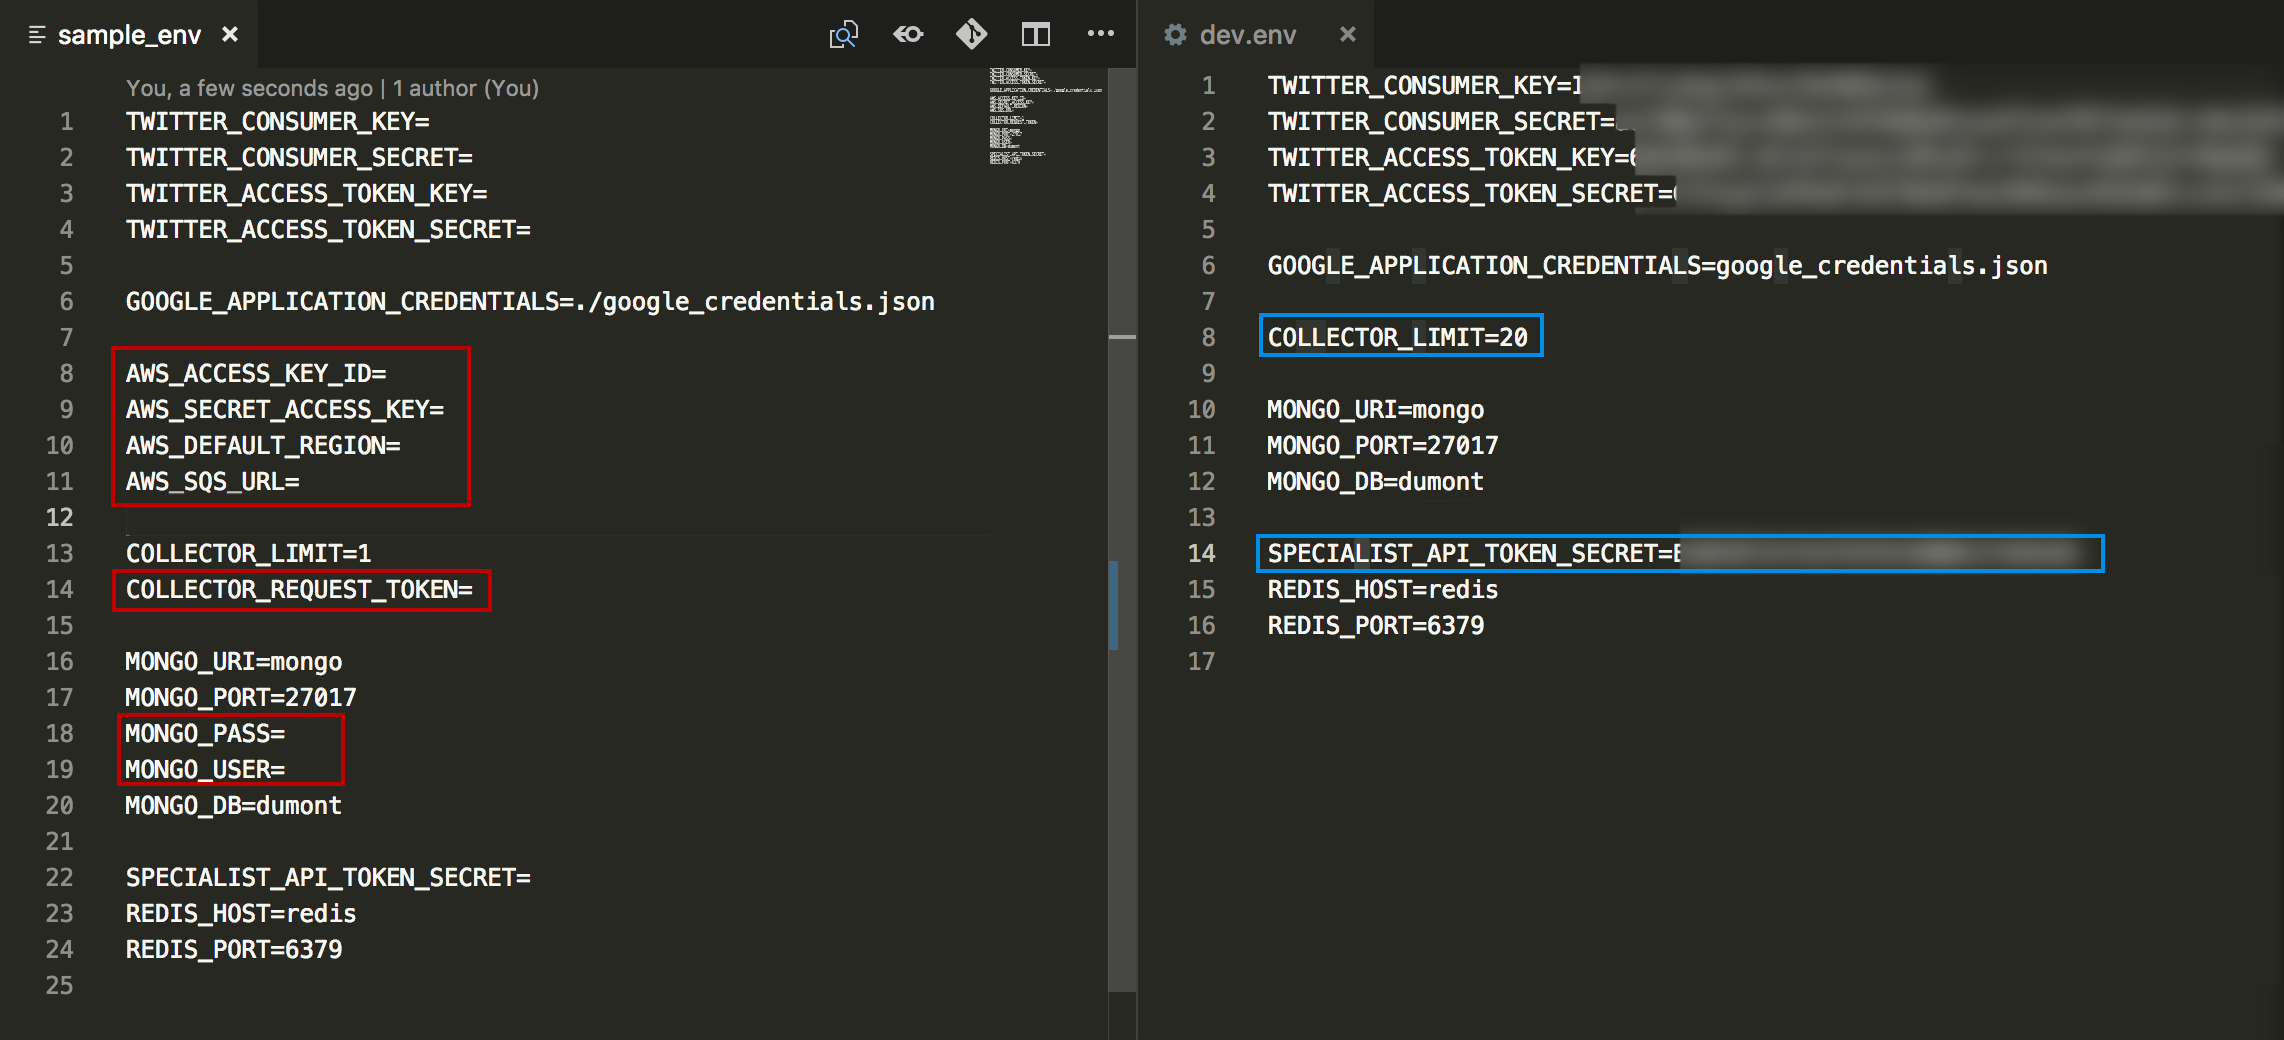
\includegraphics[width=1\textwidth]{imagens/creds.png}
    \caption{Imagem demonstrando passo a passo de como gerar o JSON de credencial}
    \label{fig:creds}
\end{figure}

É importante lembrar dos limites da API publica do twitter, e tambem que devido a implementação (que pode ser acompanhada no arquivo \textit{dumont/collector/twitter/index.js}) na linha 74 é possível ver o momento onde a \textit{stream} é parada, entretando, podem chegar inumeros tweets de diferentes usuarios simuntaneamente, fazendo assim, com que sobrecarregue a quantiadade de usuarios permitidas na API. É sugerido rodar valores baixos entre 20 a 45 para evitar problemas.

Uma vez configurado, é possivel executar o comando \textit{docker-compose -f docker-compose.dev.yml}, uma vez que o docker inicie o serviço você pode iniciar a coleta utilizando desde um navegador, ferramentas (um exemplo é o Postman\footnote{https://www.getpostman.com/}) ou até mesmo o \textit{curl} utilizando o uri \textit{\url{http://127.0.0.1:8080/}}

Depois que os dados foram coletados, ja é possível minerar algumas informações deles, para isso existem processos a serem detalhados.